% Optimization Project: Biscuit Optimizer
% Roberto Basla
% Politecnico di Milano
% A.Y. 2021/2022

\section{Further applications: histological images augmentation}
This section shows a parallel between the biscuit nesting problem and a method of data augmentation for biomedical images. Images are taken from a public dataset available on \href{https://www.kaggle.com/competitions/data-science-bowl-2018/data}{kaggle.com}.

\subsection{The augmentation problem}
Data augmentation for vision tasks in machine learning is a series of techniques used to increase the amount of data by adding slightly modified copies of already existing images or newly created synthetic data. This is an important process especially in the biomedical field, where obtaining many samples can be hard or very expensive. Figure \ref{fig:base_image} shows an image used for instance segmentation, where the objective of the learning algorithm (usually a neural network) is detecting objects of interest in an image and delineate their boundaries. The other images in Figure \ref{fig:image_masks} show some of the binary masks that represent the ground truth segmentation of one nucleus (i.e. what the algorithm has to learn).

\begin{figure}[H]
	\centering
	\begin{subfigure}[b]{.24\textwidth}
		\centering
		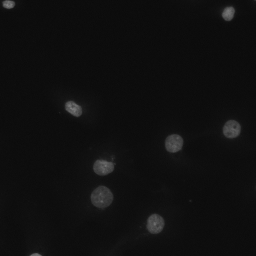
\includegraphics[width=\textwidth]{04-nuclei/base_image}
		\caption{Base image}
		\label{fig:base_image}
	\end{subfigure}
	\begin{subfigure}[b]{.24\textwidth}
		\centering
		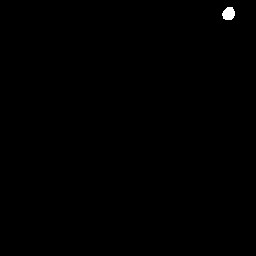
\includegraphics[width=\textwidth]{04-nuclei/mask_1}
		\caption{Ex. mask 1}
		\label{fig:mask_1}
	\end{subfigure} 
	\begin{subfigure}[b]{.24\textwidth}
		\centering
		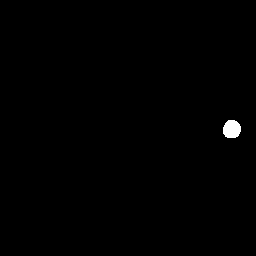
\includegraphics[width=\textwidth]{04-nuclei/mask_2}
		\caption{Ex. mask/2}
		\label{fig:mask_2}
	\end{subfigure}
	\begin{subfigure}[b]{.24\textwidth}
		\centering
		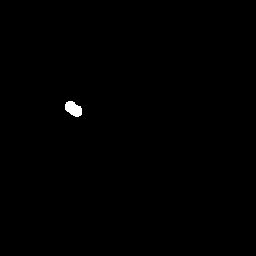
\includegraphics[width=\textwidth]{04-nuclei/mask_3}
		\caption{Ex. mask/3}
		\label{fig:mask_3}
	\end{subfigure}	
	\caption{Example image and its masks for instance segmentation}
	\label{fig:image_masks}
\end{figure}

The parallel with the problem solved by this project consists in considering the possibility of creating new (artificial) images starting from individual nuclei masks: the ground truth acts as the cookie cutters while an empty image is the biscuit dough.

\subsection{Heuristic examples}
The notebook available at \href{https://github.com/rb-sl/biscuit_optimizer/blob/main/src/04-nuclei}{src/04-nuclei} shows how an heuristic can be used to generate new nuclei images. Unfortunately, the algorithms devised in Section \ref{sec:heuristics} were not able to handle large quantities of nuclei (in the order of hundreds), therefore an ad-hoc algorithm was developed. Figure \ref{fig:aug_normal} shows a result of this process.
\begin{figure}[H]
	\centering
	\begin{subfigure}[b]{.4\textwidth}
		\centering
		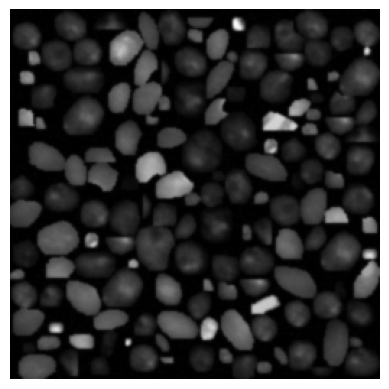
\includegraphics[width=\textwidth]{04-nuclei/aug_normal_image}
		\caption{Augmented image}
		\label{fig:aug_image}
	\end{subfigure}
	\begin{subfigure}[b]{.4\textwidth}
		\centering
		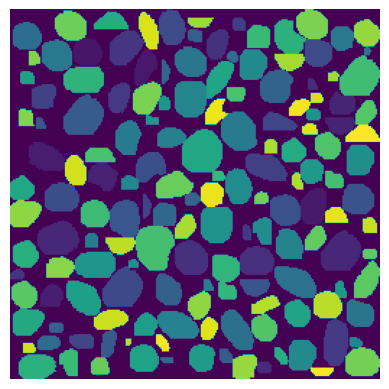
\includegraphics[width=\textwidth]{04-nuclei/aug_normal_mask}
		\caption{Augmented mask}
		\label{fig:aug_mask}
	\end{subfigure} 
	\caption{Example of augmentation}
	\label{fig:aug_normal}
\end{figure}

\subsection{Margin modification}
Augmentations usually rely on some randomization in order to create different types of images. In this context, the usage of the mask's gradient can help in enlarging or shrinking the actual nucleus mask, allowing to pack them differently and, if necessary to teach the network, overlap them. Figure \ref{fig:aug_margin} shows three examples of augmented images obtained by modifying the mask and using the previous heuristic.
\begin{figure}[H]
	\centering
	\begin{subfigure}[b]{.32\textwidth}
		\centering
		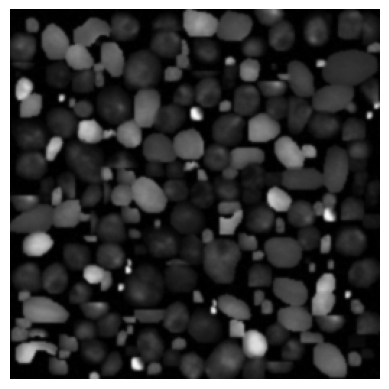
\includegraphics[width=\textwidth]{04-nuclei/aug_margin_-1}
		\caption{Lower margin (-1)}
		\label{fig:lower_margin}
	\end{subfigure}
	\begin{subfigure}[b]{.32\textwidth}
		\centering
		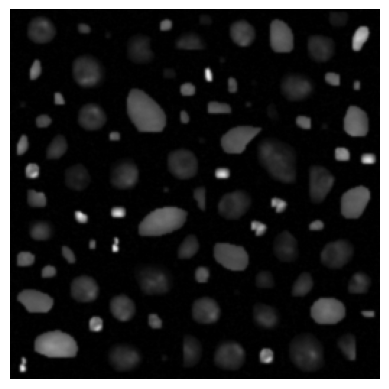
\includegraphics[width=\textwidth]{04-nuclei/aug_margin_5}
		\caption{Higher margin (+5)}
		\label{fig:higher_margin}
	\end{subfigure} 
	\begin{subfigure}[b]{.32\textwidth}
		\centering
		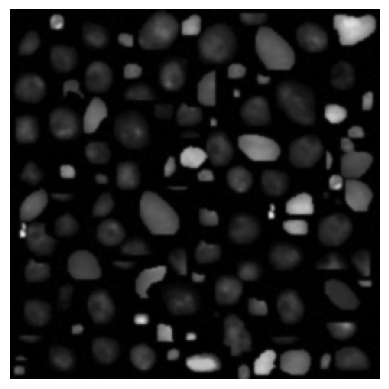
\includegraphics[width=\textwidth]{04-nuclei/aug_margin_random}
		\caption{Random margin}
		\label{fig:random_margin}
	\end{subfigure} 
	\caption{Example of augmentation with modified margins} 
	\label{fig:aug_margin}
\end{figure}
